Both the European community and Japan have proposed deep-underground
accelerator-based neutrino oscillation experiments, which overlap
significantly in motivation, technology, and physics scope with
the US neutrino 
program. There are two main proposals on the table: LAGUNA-LBNO,
a European initiative with the CERN proton beam and several potential
sites for the far detector; and T2HK, an oscillation experiment with
the JPARC beam and the HyperK target. It is important to compare the sensitivity and timescale of
these experiments with the US options. 

\subsubsection{Hyper-Kamiokande}

The Japan Subcommittee on Future HEP projects
(2012)~\cite{nonus:HEPfuture} has recommended 
that:
``Japan should aim to realize a large-scale neutrino detector ...This
new large-scale neutrino detector should have sufficient sensitivity
to allow the search for proton decays''. 
The emphasis of the program is on CP violation and proton decay, not
determination of the mass hierarchy.

The neutrinos for Japan's long-baseline program are produced at the
50 GeV proton synchrotron at J-PARC 
accelerator laboratory, in Tokai 
on the east coast of Japan. The J-PARC development plan calls for a
staged increase in proton beam power, from 300 kW presently to 1-2 MW
by the middle of the next decade~\cite{nonus:JapanMasterPlan}. 

Two primary options have been considered for the far detector:
Hyper-Kamiokande (HyperK)~\cite{nonus:HyperK}, a Megaton-scale water 
Cherenkov detector in the Kamioka region~\cite{nonus:HyperK}, 295 km
away from J-PARC; and a 100 kTon liquid argon detector at Okinoshima
island at a baseline of 660 km. As of this writing, HyperK appears
to be the front-runner. 

HyperK is a proposed very large water Cherenkov detector with a total
mass of 1 MTon. It is proposed to be located in a new detector cavity
in the Tochibora mine, about 8 km from the Super-Kamiokande location,
under an overburden of about 1750 mwe. 

The HyperK design is based on the very successful Super-Kamiokande
(SuperK) experiment, and represents a factor of 20 increase in the
fiducial mass. The extrapolation to the Megaton-scale detector will
certainly present technological challenges; however, the detector
technology and, in particular, systematic effects in  water
Cherenkov detectors are well understood. Water Cherenkov technology
offers excellent particle ID capabilities and high reconstruction
efficiency for the sub-GeV electrons and muons relevant for the
oscillation program. 

The total cost of the detector is estimated to be 50-75 Billion yen
($\approx \$500-700$M)~\cite{nonus:JapanMasterPlan}. The cost of the
neutrino beamline upgrades to provide 1-2 MW of beam power at J-PARC
is estimated at 38B yen. Thus, the long-baseline neutrino program
falls in the medium range of the future projects being considered at
Japan, between SuperKEKB/SuperBelle and the ILC. 

At the baseline of 295 km, the matter-induced neutrino mixing is
relatively small. This means a weak sensitivity to the
neutrino mass hierarchy (see Fig.~\ref{fig_four} in
Section~\ref{s:tn}). On the other hand, the sensitivity to the CP
angle $\delta_{CP}$ is enhanced compared to the matter-induced
effects. Thus, CP measurements in HyperK would require an independent
determination of the mass hierarchy. Such determination is possible
with an atmospheric neutrino campaign in HyperK, as discussed below. 

The short baseline also requires a lower neutrino energy to maintain
the detector at the first oscillation maximum. The T2HK (Tokai to HyperK)
project will utilize an off-axis, narrow-band beam similar to that of
T2K, with the 
$\nu_\mu$ energy peaking at around 600~MeV. At that energy,
backgrounds from $\nu_e$ and in particular $\nu_\tau$ are
suppressed. This configuration requires large beam power and long run
time. The HyperK proposal assumes 10 years of running at a beam power of
750~kW (3 years in neutrino and 7 years in anti-neutrino modes). 


The very large mass and significant overburden of HyperK provides the
potential for  a measurement of the neutrino mass hierarchy
with atmospheric neutrinos. 

The sensitivity of atmospheric neutrino oscillations to the neutrino
mass hierarchy is discussed in detail in Section~\ref{s:atm}. 
The sensitivity comes from the $\nu_\mu\to \nu_e$
appearance induced by the Earth matter, and thus the effect is 
strongest for upward-going neutrinos. 
In a
charge-symmetric detector like HyperK, the measurement requires
excellent identification of neutrino flavor and
precise reconstruction of neutrino energy and azimuthal angle, at
the energies of a few GeV. A water Cherenkov detector like HyperK is
well matched to these requirements. 

As discussed in
Section~\ref{s:atm}, understanding of the energy and angular
resolutions, as well as the systematics of the overall energy scale
are extremely important for extracting the mass hierarchy signal from
the atmospheric neutrino data. Unlike PINGU and other large
atmospheric neutrino detectors, with SuperK experience these
systematic effects are fairly well understood in a water Cherenkov
detector. Most importantly, HyperK will have a beam-based calibration
signal (the beam energy spectrum) and the ability to detect both
upward- and downward-going neutrinos. Those factors make the potential
for observing the neutrino mass hierarchy with atmospheric neutrinos
in HyperK quite robust. 

After 10 years of operation starting at the end of this decade
(i.e. results ready by 2028-2030), HyperK
projects to be able to determine 
the mass hierarchy with a confidence level of $2-3\sigma$ with the atmospheric
measurements, and greater than $1\sigma$ with the 
beam-based measurements alone (Fig.~\ref{fig:HyperK_sens}). The sensitivity
of the beam-based measurement depends strongly on the value of
$\delta_{CP}$ (Section~\ref{s:tn}), while the atmospheric sensitivity
depends somewhat on the value (octant) of $\theta_{23}$ and, to a
small extent, $\delta_{CP}$. 
The two
measurements are complementary, and adding them together allows HyperK
to project greater than $3\sigma$ sensitivity to the mass hierarchy for the entire
range of $\delta_{CP}$. 

\begin{figure}[bp]
\begin{center}
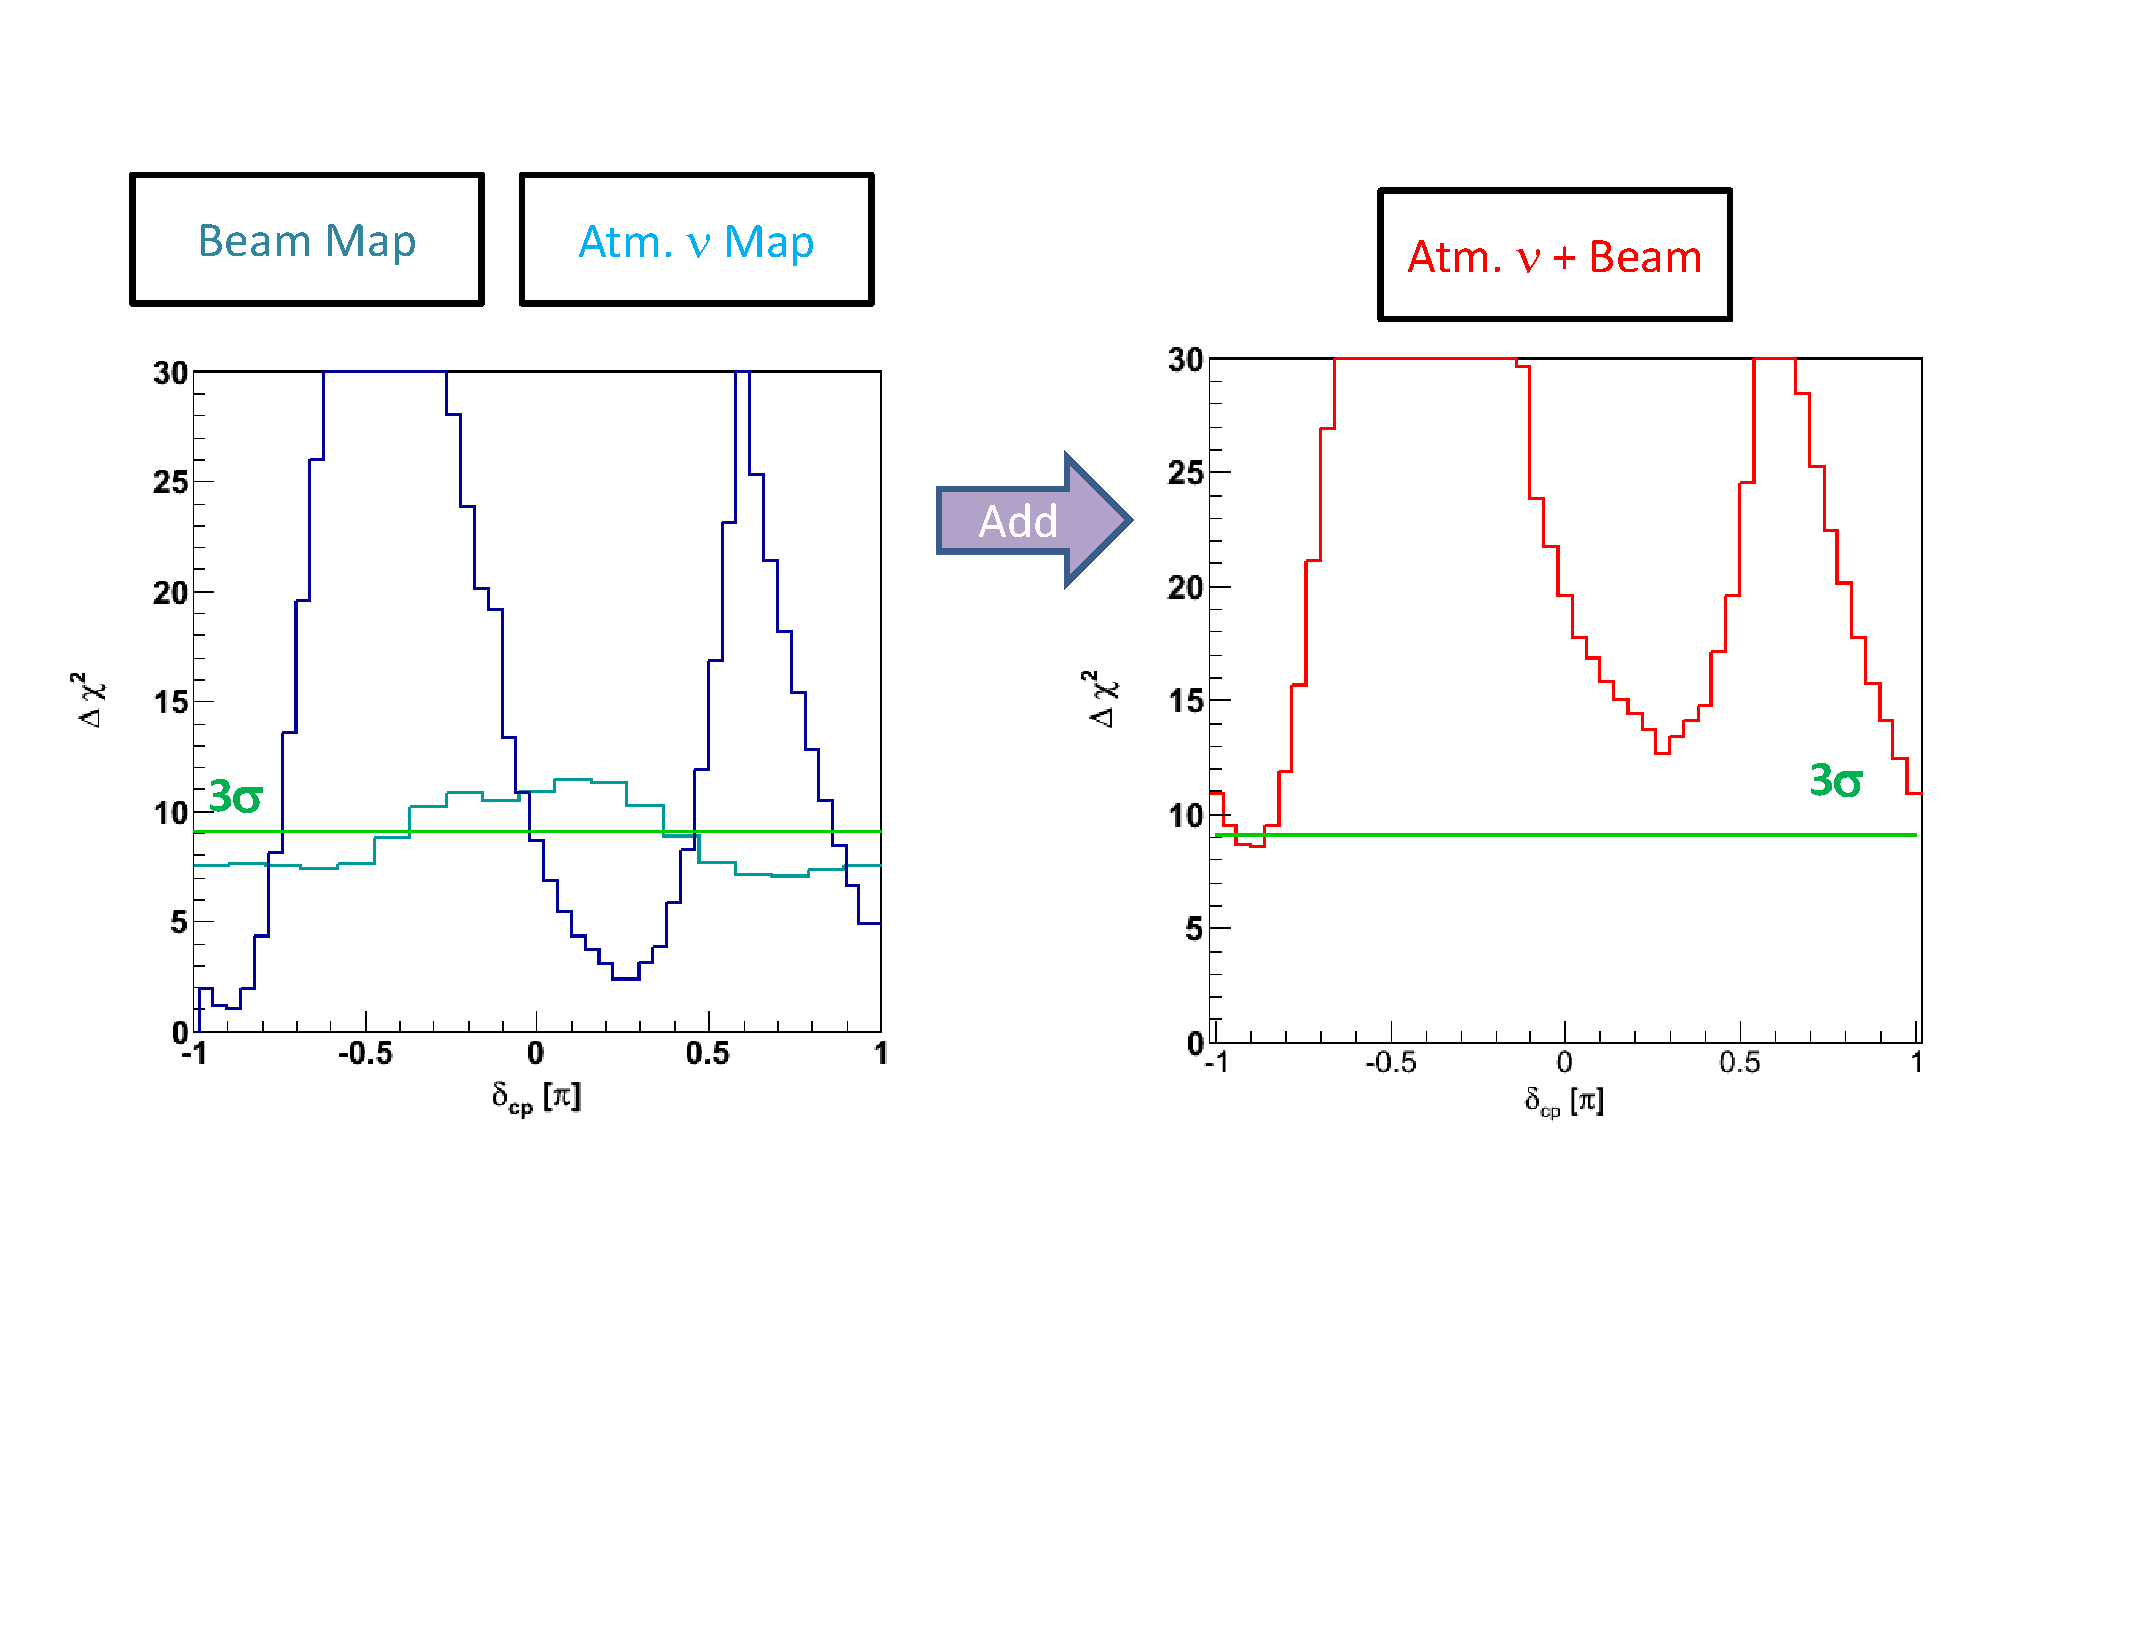
\includegraphics[width=0.9\textwidth]{YGK/HyperK.pdf}
\caption{Projected sensitivity in units of $\Delta\chi^2$ of HyperK to
  the neutrino mass 
  hierarchy from the long-baseline beam measurements (left plot, blue
  histogram) and from the atmospheric measurements (left plot,
  dark-green histogram). The combined sensitivity is shown in the
  right plot. The plot is from Ref.~\cite{nonus:HyperKsens}. } 
\label{fig:HyperK_sens}
\end{center}\end{figure}


\subsubsection{LAGUNA-LBNO}

The European version of the long-baseline neutrino oscillation
experiment is known as LAGUNA-LBNO~\cite{nonus:LAGUNA,
  nonus:EuroNuStrategy} (Large Apparatus studying Grand 
Unification and Neutrino Astrophysics and Long-Baseline Neutrino
 Oscillations).   The current cycle of design studies
(2011-2014) is focused on the conventional neutrino beam originating
at CERN, aiming at a deep underground site in Pyh\"asalmi, Finland, at
a baseline of 2300~km.  Fig.~\ref{fig_three}
illustrates the advantages of such a long baseline. 

\begin{figure}[!h]\begin{center}
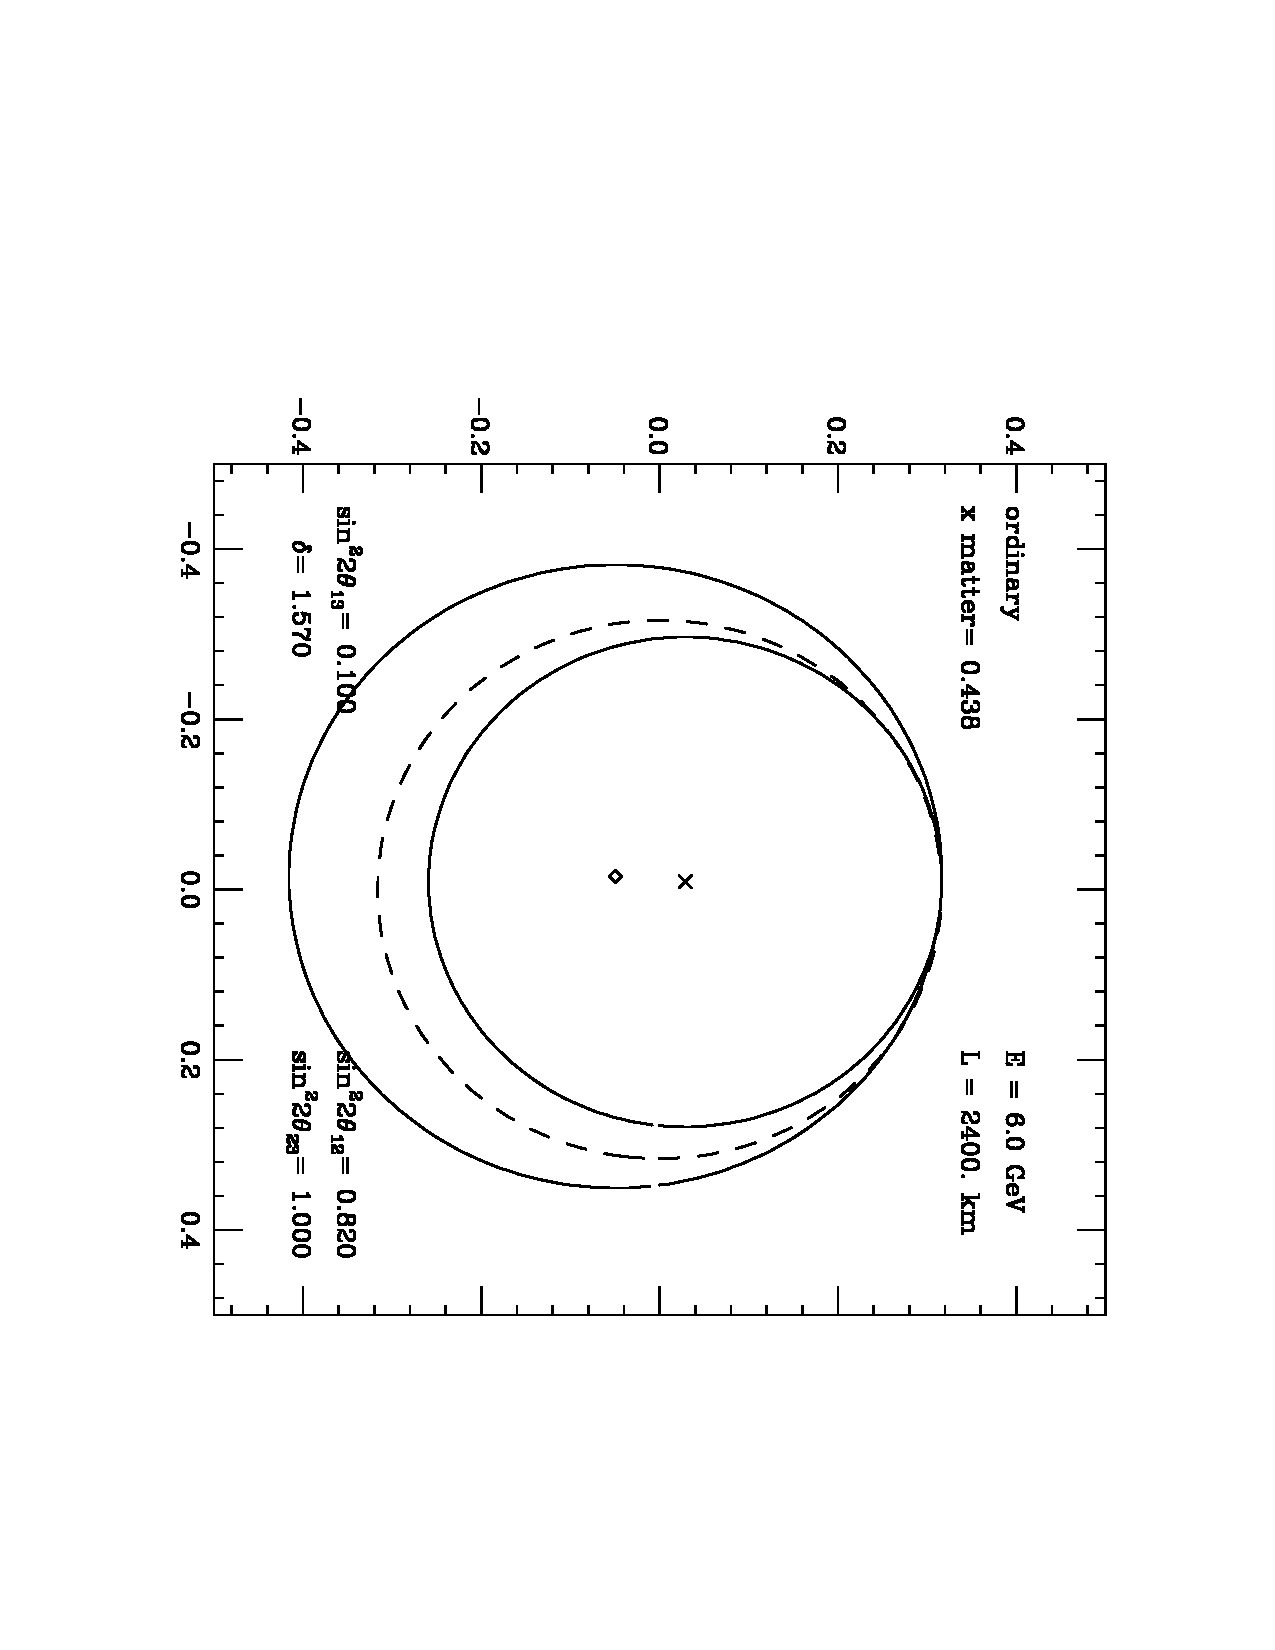
\includegraphics[width=2.45in,angle=90]{RNC/cpv_wash_pibytwo.pdf}
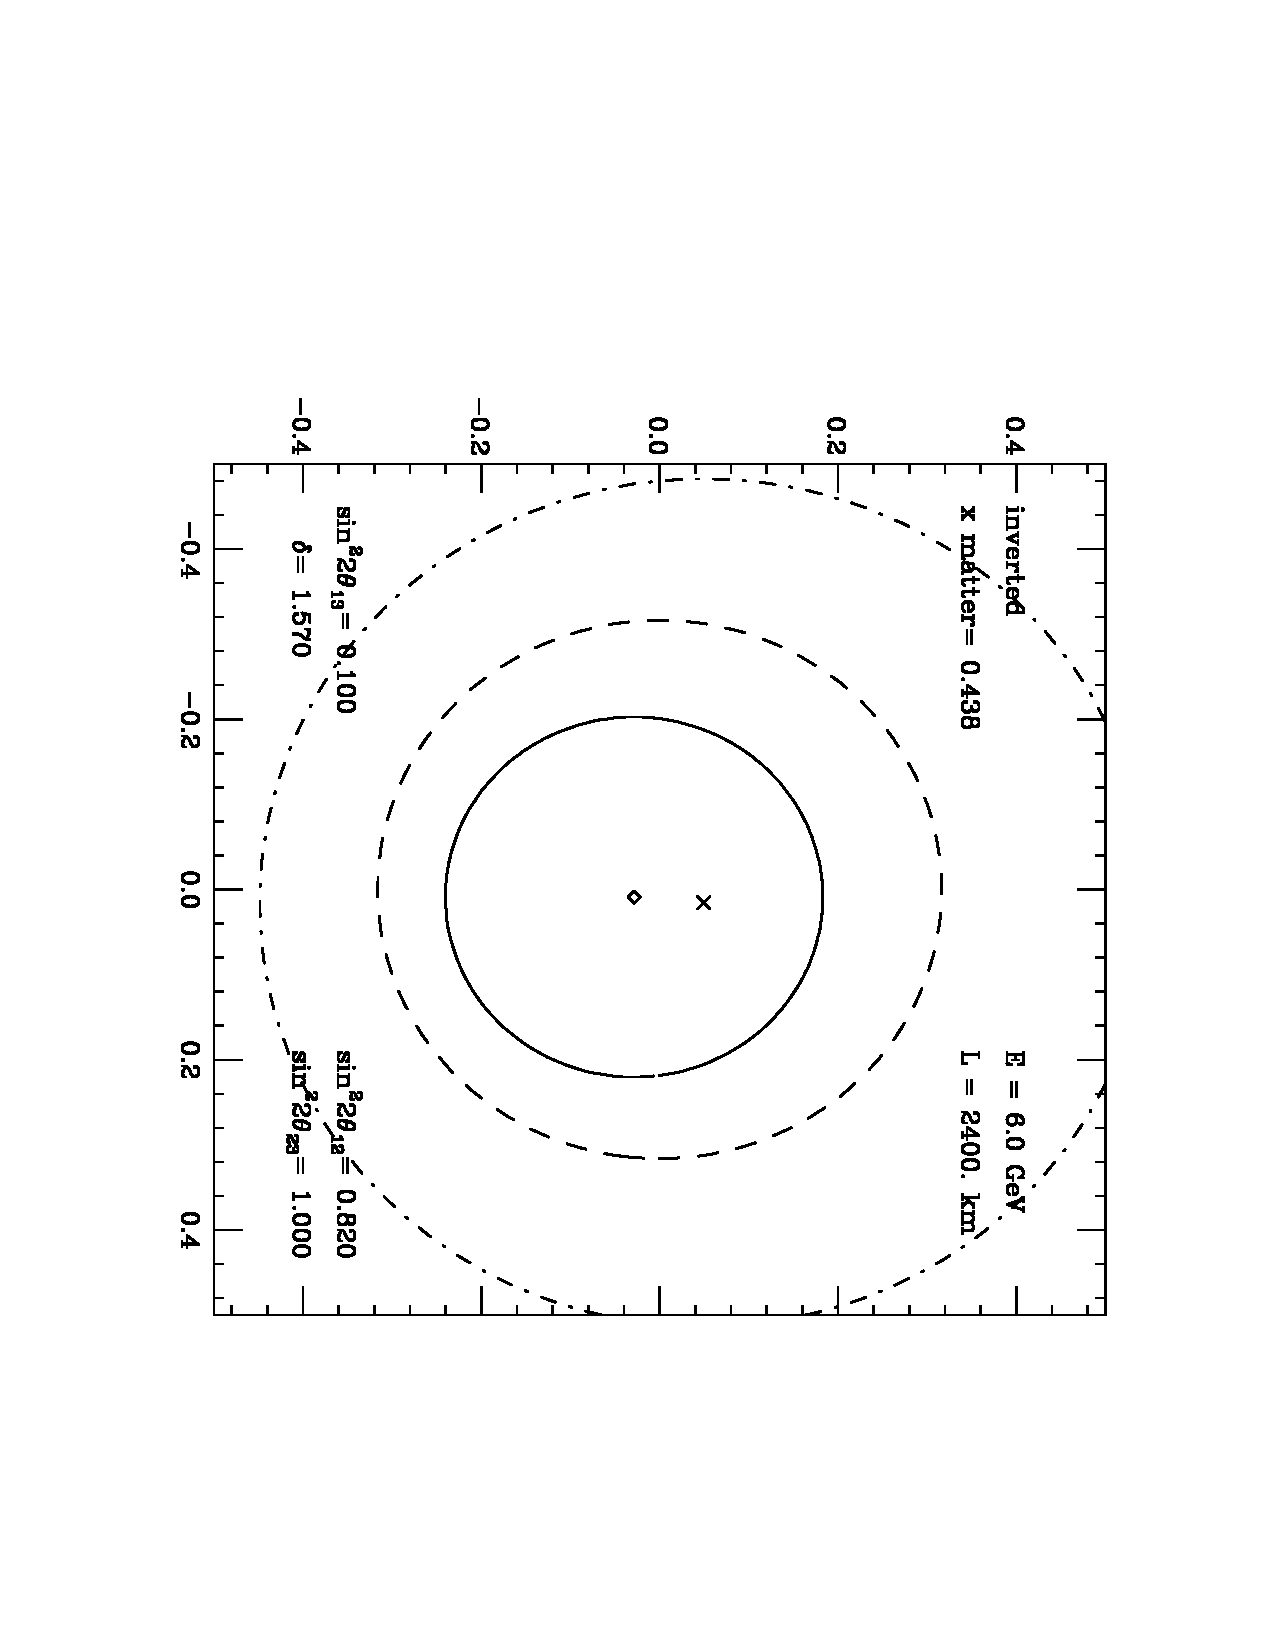
\includegraphics[width=2.45in,angle=90]{RNC/cpv_wash_pibytwo_inv.pdf}
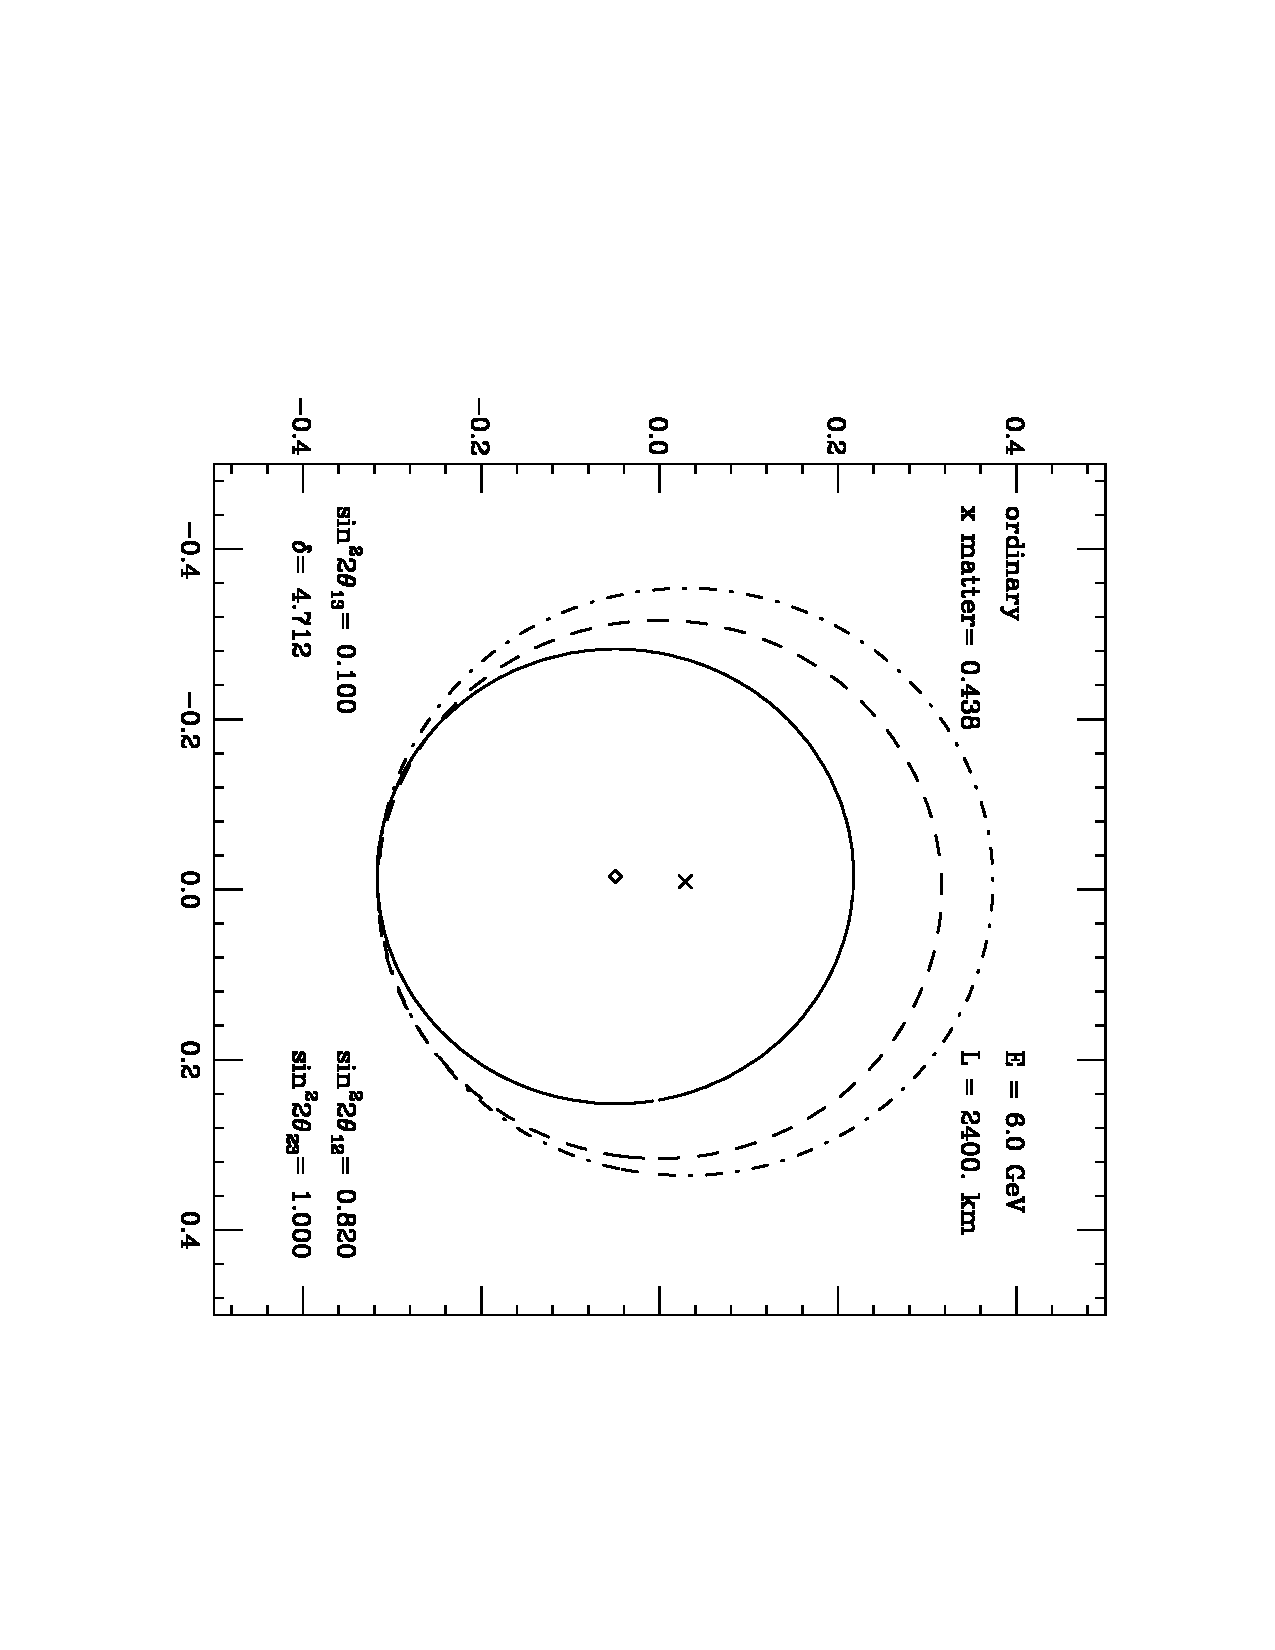
\includegraphics[width=2.45in,angle=90]{RNC/cpv_wash_threepibytwo.pdf}
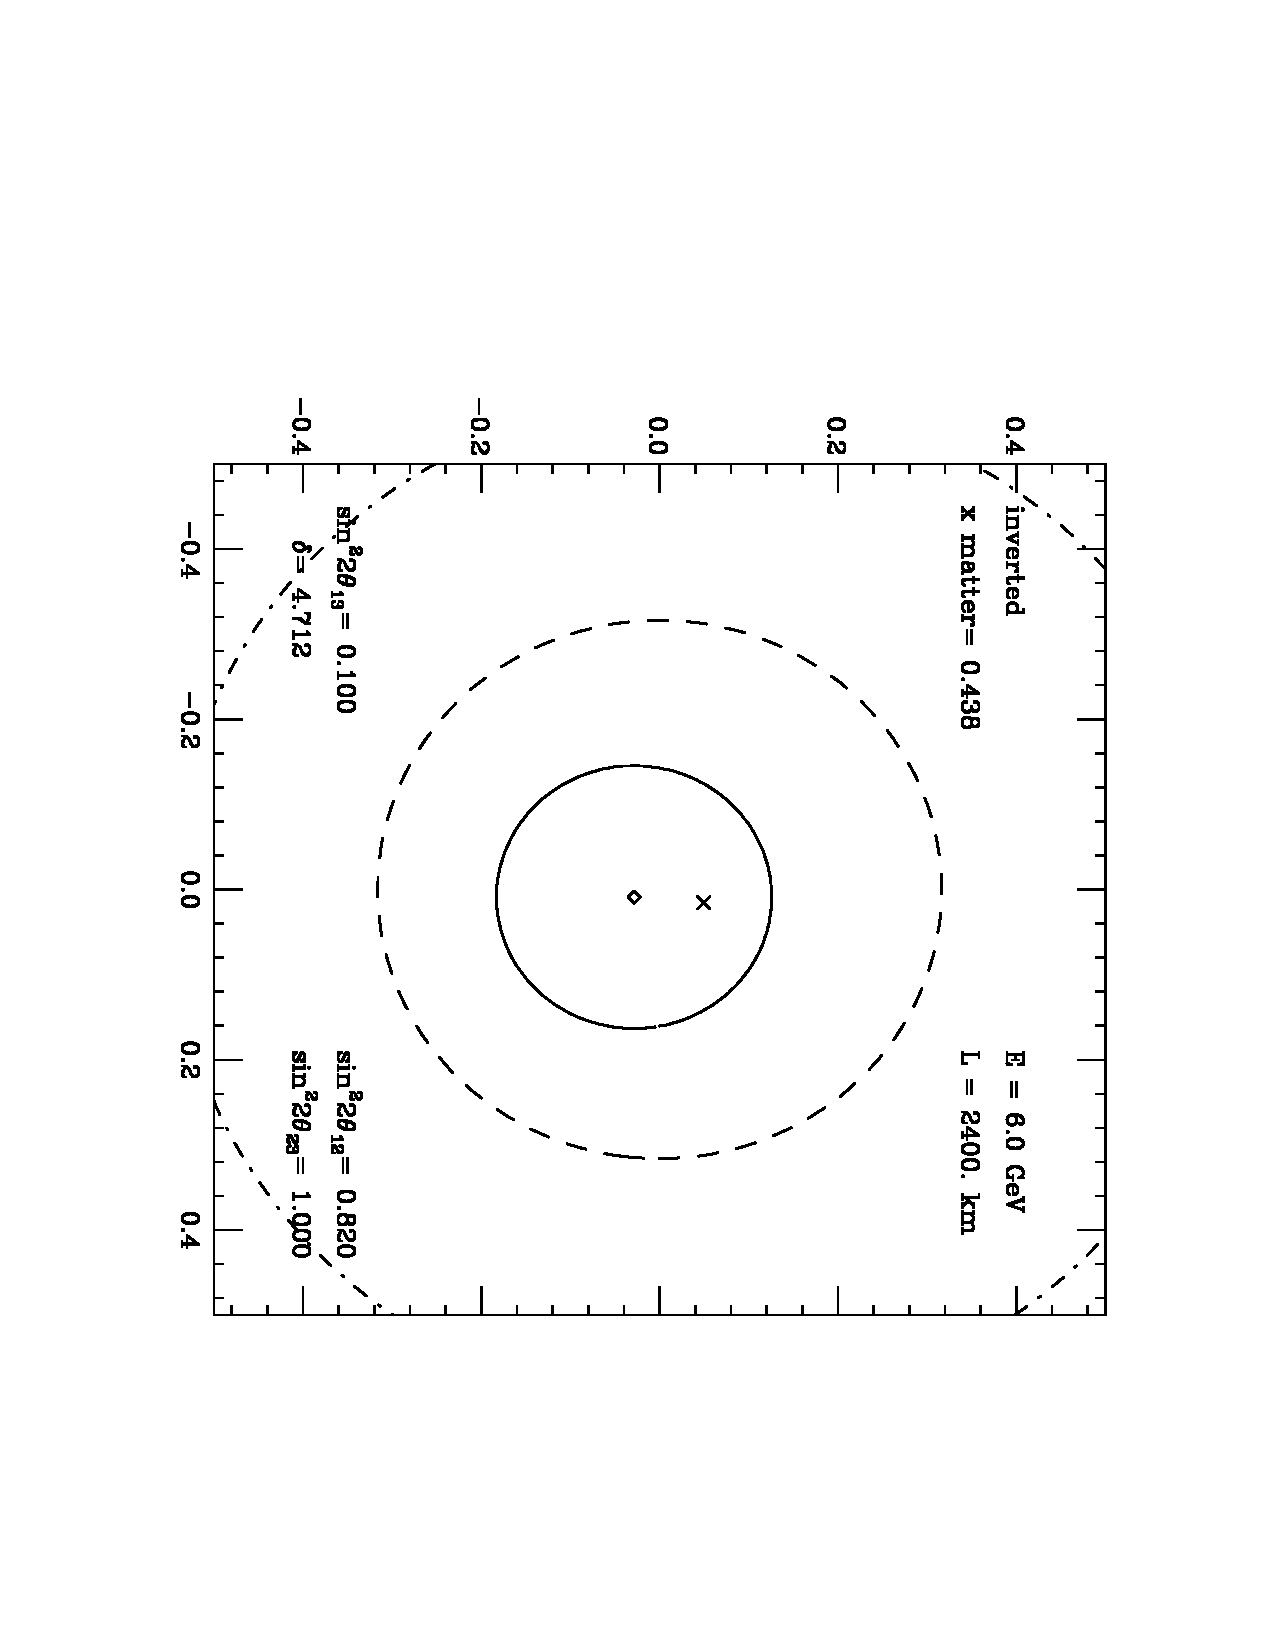
\includegraphics[width=2.45in,angle=90]{RNC/cpv_wash_threepibytwo_inv.pdf}
\caption{ Plots for a hypothetical site 2400 km from the source.  Upper, with true hierarchy being normal, with $\delta_{CP}=\pi/2$.  Lower, again with true hierarchy being normal, but now with $\delta_{CP}=3\pi/2$. The dot dash circles show the constraints from $\nu_\mu$ scattering, while the solid circles are for $\nubar_\mu$.   The dashed curve shows the constraint from reactor neutrino experiments. \label{fig_three}}
\end{center}
\vspace{-1.4cm}
\end{figure}


Three detector concepts are being developed for
that site: GLACIER (Giant Liquid Argon Charge Imaging ExpeRiment), a
LAr dual-phase TPC scalable to a total mass of up to 100 kTon; MIND,
a 25 kTon magnetized iron-scintillator calorimeter similar to
MINOS~\cite{nonus:LBNO_LOI}; and
LENA (Low Energy Neutrino Astronomy), a $\sim$50 kTon liquid
scintillator detector. In addition, a MTon-scale water Cherenkov
detector MEMPHYS (MEgaton Mass PHYSics) is being considered for a site
in an extended 
Modane Laboratory at a very short baseline of 130 km from CERN. All
cases include a near detector (upgraded SHINE/NA61), a deep
underground location (2500 mwe for GLACIER, 4000 mwe for LENA, 4800
mwe for MEMPHYS), and a range of neutrino beam options, starting with
an 800 kW wide-band beam (for GLACIER and LENA) to an upgrade to 4 MW
(for MEMPHYS), to high-power $\beta$-beams at CERN (for MEMPHYS), and
ultimately to a neutrino factory. 





Each detector offers a different set of
complementary physics measurements: GLACIER and LENA, with a very long
baseline and large underground detector, will be able to resolve the
neutrino mass hierarchy quickly, while also providing excellent CP
reach and opportunities to search for proton decay and supernova
neutrinos. The physics case for such detectors is well described in
Section~\ref{s:lb}. In addition, LENA, by virtue of its low energy
threshold, would be a large-scale solar neutrino experiment. MEMPHYS offers a different tradeoff: a clean
measurement of the CP phase $\delta_{CP}$ without significant matter
effects, increased detector mass (compared to SuperK) for proton decay
searches, and sensitivity to the mass hierarchy via measurements
of atmospheric neutrinos. The physics reach of MEMPHYS is similar to that of
HyperK. 

\begin{figure}[b]
\vspace{-0.1cm}
\begin{center}
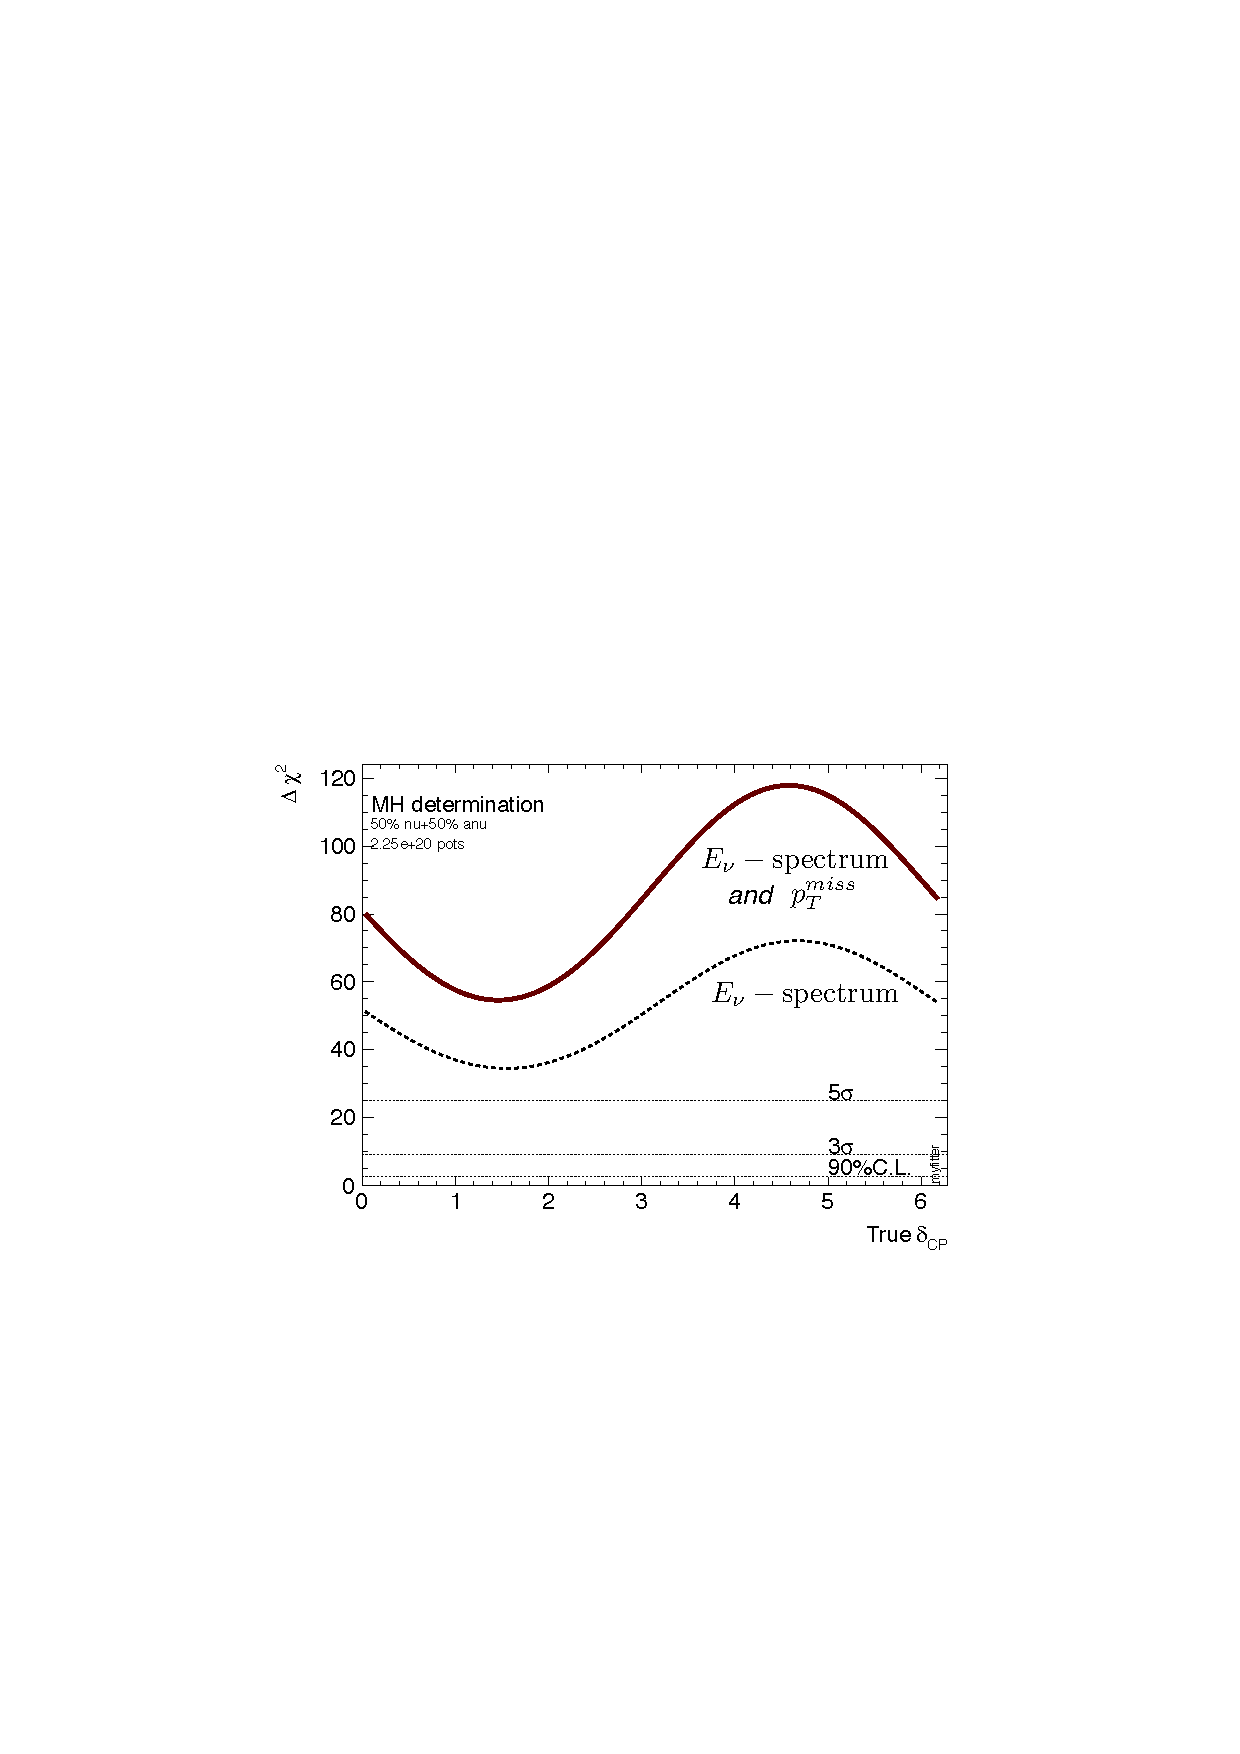
\includegraphics[width=0.47\textwidth]{YGK/LAGUNA_MH.pdf}
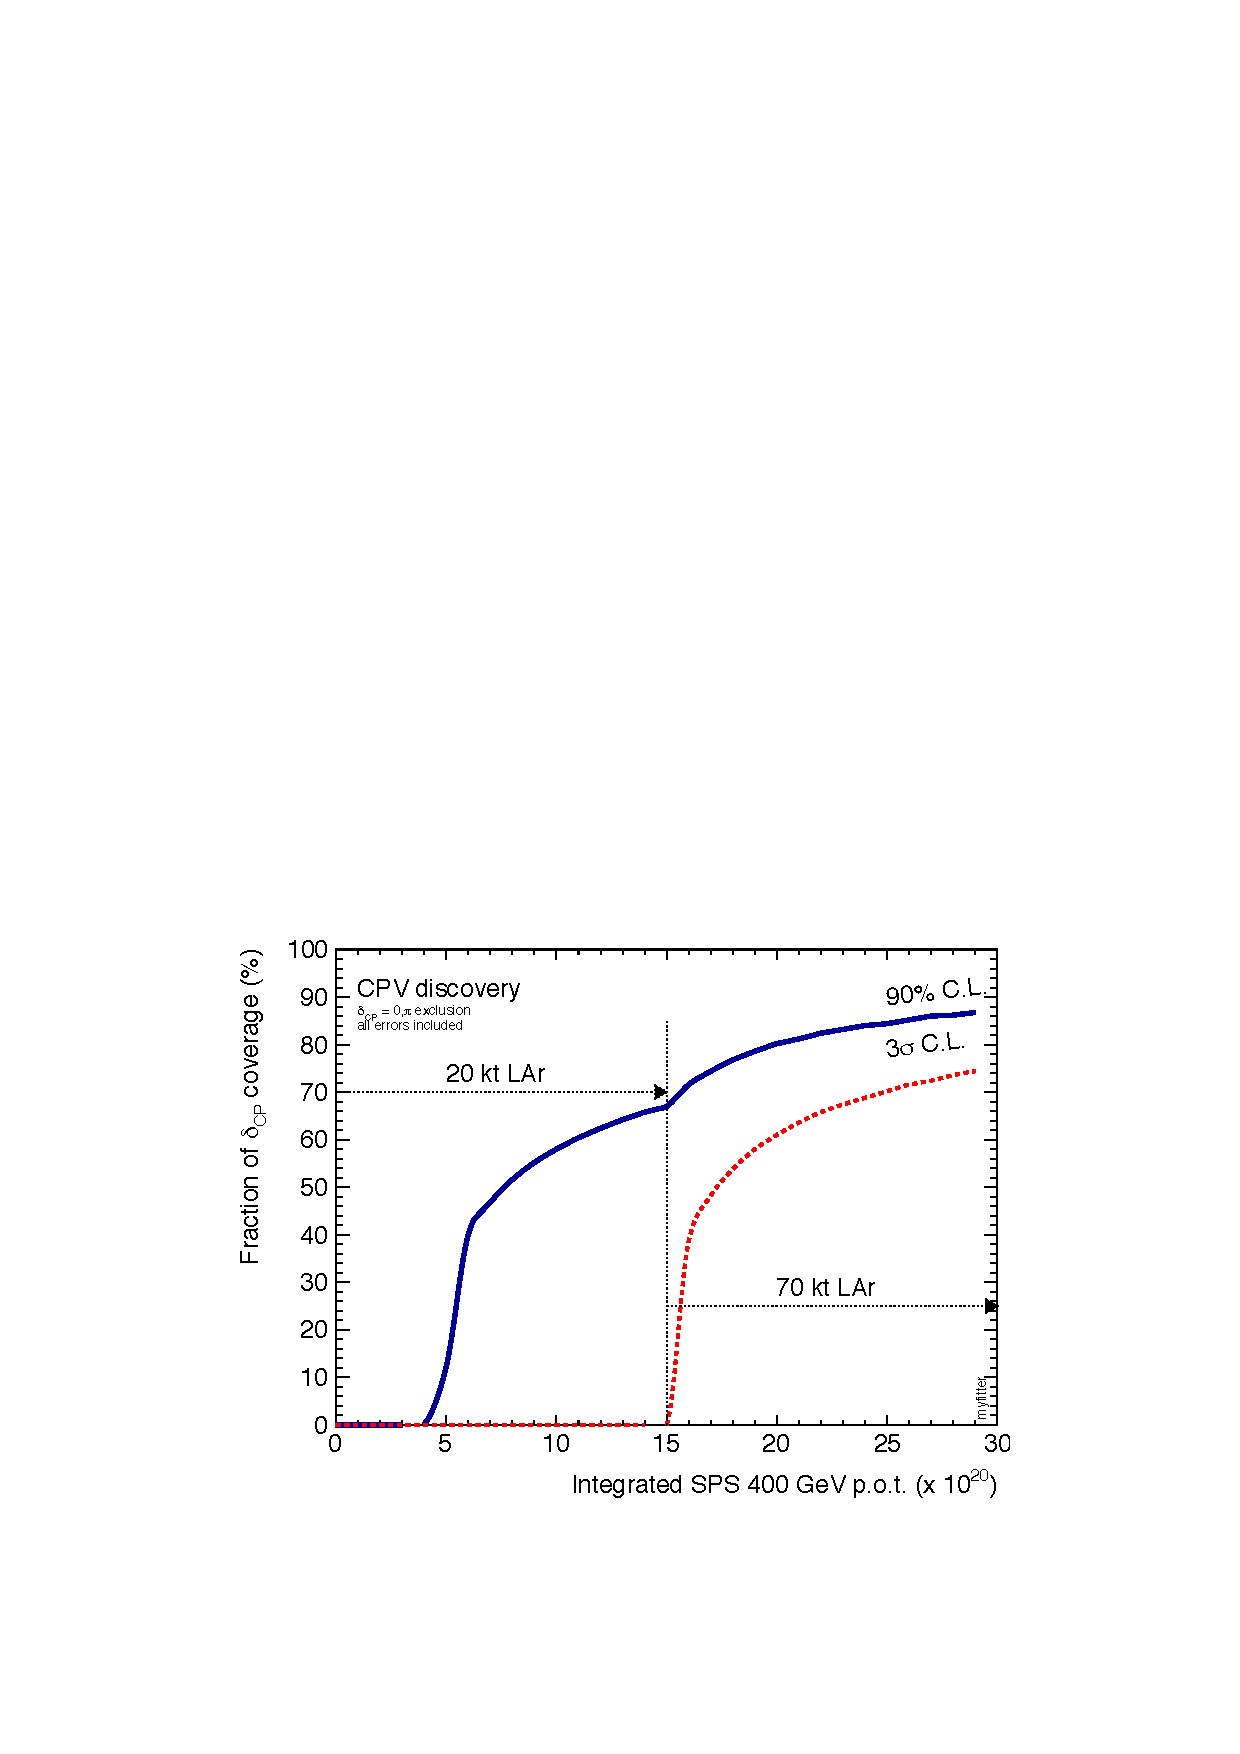
\includegraphics[width=0.47\textwidth]{YGK/LAGUNA_CP.pdf}
\caption{LAGUNA sensitivity to the mass hierarchy as a function of
  $\delta_{CP}$
  (left)~\cite{nonus:LBNO_LOI}. Sensitivity to
  $\delta_{CP}$ (right) for staged detector construction. } 
\label{fig:LAGUNA_sens}
\vspace{-0.35cm}
\end{center}\end{figure}

GLACIER, by the virtue of its excellent tracking capabilities, large
mass, and a very long baseline, can offer an extremely sensitive measurement 
of the mass hierarchy (Fig.~\ref{fig:LAGUNA_sens}). It would be able
to resolve the mass 
hierarchy with a significance of more than $5\sigma$
 in a few years of operation with a
conventional SPS beam ($\approx 2\times10^{20}$ protons on target). If
a decision on construction is reached by 
2015, the proponents estimate a $5\sigma$ measurement by
2023~\cite{nonus:EuroNuStrategy,nonus:LBNO_LOI}. The high sensitivity
would possibly enable a staged 
approach to the project: a smaller (20 kTon) detector that starts operating
quickly, followed by a larger detector, near detector upgrades, beam
intensity upgrades, etc, aiming at a 30-year program for precision
measurement of $\delta_{CP}$, neutrino astrophysics, and proton
decay searches.  
LENA would require about 10 years of operations to reach $>5\sigma$
sensitivity to the mass hierarchy, with the completion timescale similar
to that of LBNE and HyperK. 

While LAGUNA-LBNO claims the best sensitivity to the mass hierarchy
among the options we have considered, it is not yet a fully
fleshed-out project. The current study of the detector configuration
options is funded through 2014, at which point the proponents are
planning to submit a full proposal to
CERN~\cite{nonus:LAGUNA,nonus:EuroNuStrategy}. As of 
this writing, no cost estimates are available, although one could
scale from LBNE and HyperK estimates and come up with numbers in the range of a
few billion Euro. At that scale, the neutrino projects will be
in direct competition with the LHC upgrades, any proposals for a
high-energy $e^+e^-$ collider, etc. The recently updated 2013 European
Strategy for Particle Physics document~\cite{nonus:EuroNuStrategy}
lists neutrino physics as priority \#4 (last) and states: 
\begin{quotation} ``CERN should 
develop a neutrino programme to pave the way for 
a substantial European role in future long-baseline 
experiments. Europe should explore the possibility 
of major participation in leading long-baseline 
neutrino projects in the US and Japan''.\end{quotation} Taken at face value, this
indicates a luke-warm interest for an expensive neutrino project in
Europe, although other opinions exist. 

\subsubsection{Open Concerns}

The biggest concern for the long-baseline projects in Japan and Europe
is the fact that these projects are not fully funded in
their host countries, and so they remain virtual for now. It is
difficult to imagine the world-wide scientific community supporting
more than one expensive long-baseline effort, especially in the face
of other priorities in high energy physics. The European
Strategy document seems to openly acknowledge this fact. However,
should the US LBNE effort falter, or should the political and economic
climates change, the off-shore projects may provide viable
alternatives (and in some scenarios stiff competition) to LBNE in the
race to unambiguously and decisively determine the neutrino mass
hierarchy. 
